
%%%%%%%%%%%%%%%%%%%%%%%%%%%%%%%%%%%%%%%%%%%%%%%%%%%%%%%%%%%%%%%%%%%%%%%%%%%%%%%%
\documentclass[letterpaper, 10pt, conference]{ieeeconf}

\IEEEoverridecommandlockouts
\overrideIEEEmargins

\usepackage{mathtools}
\usepackage{mathrsfs}
\usepackage{cite}
\usepackage{amsmath}
\usepackage{amssymb}
\usepackage{amsfonts}
\usepackage{graphicx}
\usepackage{adjustbox}
\usepackage{xcolor}
\usepackage{booktabs}
\usepackage[thmmarks, amsmath]{ntheorem}

\DeclareMathOperator{\diff}{d}
\newcommand{\ddt}{\tfrac{\diff}{\diff \! t}}
\providecommand{\norm}[1]{\lVert#1\rVert}

\newtheorem{theorem}{Theorem}
\newtheorem{lemma}{Lemma}
\newtheorem{proposition}{Proposition}
\newtheorem{assumption}{Assumption}
\newtheorem{remark}{Remark}
\newtheorem{definition}{Definition}
\newtheorem{corollary}{Corollary}

\title{\LARGE \bf
Impedance and Admittance Control of a 2-DOF Robot Arm
}

\author{Ashvin Anilkumar, Leo Xu}

\begin{document}

\maketitle
\thispagestyle{plain}
\pagestyle{plain}

%%%%%%%%%%%%%%%%%%%%%%%%%%%%%%%%%%%%%%%%%%%%%%%%%%%%%%%%%%%%%%%%%%%%%%%%%%%%%%%%

\begin{figure}[htbp]
    \centering
    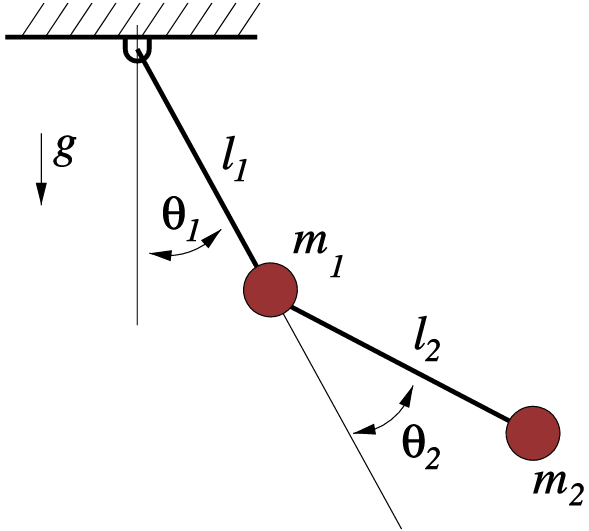
\includegraphics[width=0.25\textwidth]{simple_double_pend.png}
    \caption{Diagram of 2-DOF robot arm \cite{underactuated}.}
    \label{fig:arm}
\end{figure}

\section{Introduction \& Motivation}

A robot that touches its environment must regulate
the relationship between motion and contact force,
not motion alone. In this project, we study this
problem on the 2-DOF robot arm shown in
Figure~\ref{fig:arm}. Its equations of motion
contain nonlinear terms (sines and cosines) and
make it a simple but representative manipulator.

Our primary goal is to design and analyze a
torque-based \emph{impedance controller}
\cite{hogan1985impedance}, which makes the arm
behave like a virtual spring-damper about a desired
trajectory. We will (i) derive and linearize the
open-loop dynamics, (ii) show how the impedance law
changes the local dynamics and stability, and
(iii) evaluate the controller in simulation under
reference changes and external disturbance torques.
If time permits, our secondary goal is to design a
position-based \emph{admittance controller}, the
dual of impedance control, and compare the two.

\section{Mathematical Model \& Linearization}

As given by \cite{underactuated}, the equations
of motion (EOM) for a general robotic manipulator
with joint position vector $\mathbf{q}$,
where $\dim(\mathbf{q})=n$, are

\begin{equation}
\boxed{
\mathbf{M}(\mathbf{q})\ddot{\mathbf{q}}
+
\mathbf{C}(\mathbf{q},\dot{\mathbf{q}})
\dot{\mathbf{q}}
=
\boldsymbol{\tau}_g(\mathbf{q})
+
\mathbf{B}\mathbf{u}
+
\boldsymbol{\tau}_{\mathrm{ext}}.
}
\label{eq:eom}
\end{equation}

Here,
$\mathbf{M}(\mathbf{q})\in\mathbb{R}^{n\times n}$
is the inertia matrix,
$\mathbf{C}(\mathbf{q},\dot{\mathbf{q}})
\in\mathbb{R}^{n\times n}$
captures Coriolis and centrifugal effects,
$\boldsymbol{\tau}_g(\mathbf{q})\in\mathbb{R}^{n}$
is the gravitational torque vector,
$\mathbf{B}\in\mathbb{R}^{n\times m}$
maps the control inputs
$\mathbf{u}\in\mathbb{R}^{m}$
to generalized forces, and
$\boldsymbol{\tau}_{\mathrm{ext}}\in\mathbb{R}^{n}$
is an external (contact) torque, which is zero in
free motion. Compared with \cite{underactuated}, the
term $\boldsymbol{\tau}_{\mathrm{ext}}$ is added so
that interaction with the environment can be studied.

For the simple 2-DOF example
\cite{underactuated}, we have

\[
\adjustbox{max width=0.95\columnwidth}{$\displaystyle
\mathbf{M}(\mathbf{q}) =
\begin{bmatrix}
(m_1+m_2)l_1^2 + m_2l_2^2 + 2m_2l_1l_2c_2
&
m_2l_2^2 + m_2l_1l_2c_2
\\[6pt]
m_2l_2^2 + m_2l_1l_2c_2
&
m_2l_2^2
\end{bmatrix}
$}
\]

\[
\adjustbox{max width=0.95\columnwidth}{$\displaystyle
\mathbf{C}(\mathbf{q},\dot{\mathbf{q}}) =
\begin{bmatrix}
0
&
-m_2l_1l_2(2\dot{q}_1+\dot{q}_2)s_2
\\[6pt]
\frac{1}{2}m_2l_1l_2(2\dot{q}_1+\dot{q}_2)s_2
&
-\frac{1}{2}m_2l_1l_2\dot{q}_1s_2
\end{bmatrix}
$}
\]

\[
\adjustbox{max width=0.95\columnwidth}{$\displaystyle
\boldsymbol{\tau}_g(\mathbf{q}) =
-g
\begin{bmatrix}
(m_1+m_2)l_1s_1 + m_2l_2s_{1+2}
\\[6pt]
m_2l_2s_{1+2}
\end{bmatrix}
$}
\]

\[
\mathbf{B} =
\begin{bmatrix}
1 & 0\\
0 & 1
\end{bmatrix}
=\mathbf{I}_2,
\]

so both joints are directly actuated. Here, we use
the shorthand notation

\begin{align*}
c_2 &= \cos(q_2), &
s_1 &= \sin(q_1),\\
s_2 &= \sin(q_2), &
s_{1+2} &= \sin(q_1+q_2).
\end{align*}

For strictly positive masses and link lengths,
$\mathbf{M}(\mathbf{q})$ is positive definite
and therefore invertible, so

\begin{equation}
\adjustbox{max width=0.80\columnwidth}{$\displaystyle
\ddot{\mathbf{q}} =
\mathbf{M}(\mathbf{q})^{-1}
\left[
-\mathbf{C}(\mathbf{q},\dot{\mathbf{q}})
\dot{\mathbf{q}}
+\mathbf{B}\mathbf{u}
+\boldsymbol{\tau}_g(\mathbf{q})
+\boldsymbol{\tau}_{\mathrm{ext}}
\right].
$}
\label{eq:acceleration}
\end{equation}

\subsection{Open-Loop Linearization}

Define the state $\mathbf{x} =
[q_1\ q_2\ \dot{q}_1\ \dot{q}_2]^{T}$ and the
control $\mathbf{u} = [\tau_1\ \tau_2]^{T}$, with
$\boldsymbol{\tau}_{\mathrm{ext}}=\mathbf{0}$. The
dynamics take the form
$\dot{\mathbf{x}}=\mathbf{f}(\mathbf{x},\mathbf{u})$,
and the output is the pair of joint positions,
$\mathbf{y}=\mathbf{C}_y\mathbf{x}$ with
$\mathbf{C}_y=[\mathbf{I}_2\ \ \mathbf{0}_{2\times2}]$.

We linearize about the downward-hanging equilibrium
$\mathbf{x}^*=\mathbf{0}$, $\mathbf{u}^*=\mathbf{0}$,
where $\mathbf{f}(\mathbf{x}^*,\mathbf{u}^*)=\mathbf{0}$.
With $\delta\mathbf{x}=\mathbf{x}-\mathbf{x}^*$ and
$\delta\mathbf{u}=\mathbf{u}-\mathbf{u}^*$, the
first-order Taylor approximation gives

\begin{equation}
\boxed{
\delta\dot{\mathbf{x}}
=
\mathbf{A}\delta\mathbf{x}
+
\mathbf{B}_{\mathrm{lin}}\delta\mathbf{u},
}
\label{eq:linear_ss}
\end{equation}

with $\mathbf{A}=\partial\mathbf{f}/\partial\mathbf{x}$
and $\mathbf{B}_{\mathrm{lin}}=
\partial\mathbf{f}/\partial\mathbf{u}$ evaluated at
the equilibrium. Because the Coriolis terms are
quadratic in velocity, they vanish in the
linearization, and we obtain

\[
\adjustbox{max width=0.95\columnwidth}{$\displaystyle
\mathbf{A} =
\begin{bmatrix}
0&0&1&0\\[4pt]
0&0&0&1\\[4pt]
-\dfrac{g}{l_1}
&
\dfrac{gm_2}{m_1l_1}
&0&0\\[10pt]
\dfrac{g}{l_1}
&
-\dfrac{g[m_1l_1+m_2(l_1+l_2)]}
{m_1l_1l_2}
&0&0
\end{bmatrix}
$}
\]

\[
\adjustbox{max width=0.95\columnwidth}{$\displaystyle
\mathbf{B}_{\mathrm{lin}} =
\frac{1}{m_1m_2l_1^2l_2^2}
\begin{bmatrix}
0&0\\
0&0\\
m_2l_2^2&-m_2l_2(l_1+l_2)\\
-m_2l_2(l_1+l_2)&
m_1l_1^2+m_2(l_1+l_2)^2
\end{bmatrix}.
$}
\]

This $\mathbf{A}$ has the block form
$\begin{bsmallmatrix}\mathbf{0}&\mathbf{I}\\
\mathbf{K}_g&\mathbf{0}\end{bsmallmatrix}$ with
$\mathbf{K}_g$ negative definite, so we expect purely
imaginary eigenvalues: the undamped arm is only
marginally stable, and the linearization alone cannot
decide stability of the nonlinear system. We will
confirm this numerically and also check
controllability and observability. This motivates
feedback that adds damping.

\section{Impedance Control (Primary Goal)}

Let $\mathbf{q}_d$ be a desired (constant) joint
configuration. We apply the torque law

\begin{equation}
\boxed{
\mathbf{u} =
\boldsymbol{\tau}_g(\mathbf{q})
+\mathbf{K}(\mathbf{q}_d-\mathbf{q})
-\mathbf{D}\dot{\mathbf{q}},
}
\label{eq:impedance}
\end{equation}

where $\mathbf{K},\mathbf{D}\in\mathbb{R}^{2\times2}$
are symmetric positive definite stiffness and damping
gains. Gravity is compensated, and the remaining
terms act as a virtual spring-damper at each joint.
Substituting into~\eqref{eq:eom} gives the closed
loop

\[
\mathbf{M}(\mathbf{q})\ddot{\mathbf{q}}
+\left(\mathbf{C}(\mathbf{q},\dot{\mathbf{q}})
+\mathbf{D}\right)\dot{\mathbf{q}}
+\mathbf{K}(\mathbf{q}-\mathbf{q}_d)
=\boldsymbol{\tau}_{\mathrm{ext}}.
\]

With error $\mathbf{e}=\mathbf{q}-\mathbf{q}_d$ and
state $\mathbf{z}=[\mathbf{e}^{T}\ \dot{\mathbf{e}}^{T}]^{T}$,
linearizing about $\mathbf{z}=\mathbf{0}$,
$\boldsymbol{\tau}_{\mathrm{ext}}=\mathbf{0}$ yields

\begin{equation}
\dot{\mathbf{z}} =
\underbrace{\begin{bmatrix}
\mathbf{0} & \mathbf{I}\\
-\mathbf{M}_d^{-1}\mathbf{K} & -\mathbf{M}_d^{-1}\mathbf{D}
\end{bmatrix}}_{\mathbf{A}_{cl}}\mathbf{z}
+
\begin{bmatrix}
\mathbf{0}\\ \mathbf{M}_d^{-1}
\end{bmatrix}\boldsymbol{\tau}_{\mathrm{ext}},
\label{eq:closed_loop}
\end{equation}

where $\mathbf{M}_d=\mathbf{M}(\mathbf{q}_d)$. This is
a mass-spring-damper whose stiffness and damping we
choose. Because $\mathbf{M}_d$, $\mathbf{K}$, and
$\mathbf{D}$ are positive definite, $\mathbf{A}_{cl}$
is Hurwitz. We will verify this numerically. To keep
the project tractable, we use diagonal gains and
simulate in joint space only.

\subsection*{Planned analysis and simulation}

\begin{itemize}
\item Eigenvalues of $\mathbf{A}_{cl}$ for a few
choices of $\mathbf{K}$ and $\mathbf{D}$ at one or two
values of $\mathbf{q}_d$.
\item Nonlinear simulation (numerical ODE
integration): step in $\mathbf{q}_d$ and a short
disturbance torque pulse $\boldsymbol{\tau}_{\mathrm{ext}}$,
compared against the linear model.
\item Effect of stiffness versus damping on the
response.
\end{itemize}

\section{Admittance Control (If Time Permits)}

Admittance control is the dual of impedance control:
a measured external torque is mapped to a motion
offset, which is tracked by a stiff position loop. A
virtual mass-spring-damper

\begin{equation}
\mathbf{M}_v\ddot{\mathbf{x}}_v
+\mathbf{D}_v\dot{\mathbf{x}}_v
+\mathbf{K}_v\mathbf{x}_v
=\boldsymbol{\tau}_{\mathrm{ext}},
\qquad
\mathbf{q}_d=\mathbf{q}_{\mathrm{target}}+\mathbf{x}_v,
\label{eq:admittance}
\end{equation}

generates the commanded position, which is passed as
$\mathbf{q}_d$ to a high-gain version of the inner loop
in~\eqref{eq:impedance}. The system input is then a
commanded position rather than a torque. This reuses
the impedance controller as the inner loop, so it adds
only one extra filter. We would run the same
disturbance scenario as before and compare the two
responses.

\section{Plan \& Deliverables}

\begin{table}[htbp]
\centering
\caption{Proposed timeline.}
\begin{tabular}{@{}ll@{}}
\toprule
Stage & Task \\
\midrule
1 & Model, linearize, and verify numerically \\
2 & Open-loop eigenvalue, controllability, observability \\
3 & Impedance controller, closed-loop analysis, simulation \\
4 & (Optional) Admittance controller and comparison \\
5 & Final report and presentation \\
\bottomrule
\end{tabular}
\end{table}

We will implement the nonlinear model and controllers
in Python (NumPy/SciPy) and report the open-loop and
closed-loop eigenvalues and the step and disturbance
responses for a few gain choices. Success means a
stable, well-damped closed loop that tracks
$\mathbf{q}_d$ and deflects predictably under
$\boldsymbol{\tau}_{\mathrm{ext}}$. All work is in
simulation, with no hardware.

\bibliographystyle{IEEEtran}
\bibliography{mybibfile}

\end{document}
